\documentclass[11pt, aspectratio=169]{beamer}
%%%%%%%%%%%%%%%%%%%%%%%%%%%%%%%%%%%%%%%%%%%%%%%%%%%%%%
%%%%%%%%%%%%%%%%%%%%%%%%%%%%%%%%%%%%%%%%%%%%%%%%%%%%%%%%%%%%%%%%
%%%%%%%%%%%%%%%%%%%%%%%%%%%%%%%%%%%%%%%%%%%%%%%%%%%%%%%%%%%%%%%%%%%%%%%%%%%%%%%%%%%%%%%%%%%%%%%%%%%%%%%%%%%%%%%%%%%%%%%%%%%%%%%%%%%%%%
\usepackage{hyperref}
\usepackage{etex}
\usepackage{morewrites}
\usepackage{epsf,psfrag,float}
\usepackage{multirow,hhline, subfigure, epsfig,graphpap,pspicture,float}
\usepackage{colortbl}
\usepackage{threeparttable}
\usepackage{booktabs}
\usepackage{seqsplit}
\usepackage{tabularx}
\usepackage{multirow}
\usepackage{dcolumn}
\newcolumntype{.}{D{.}{.}{-1}}
\usepackage{adjustbox}
\setcounter{secnumdepth}{3}
\setcounter{tocdepth}{3}
\usepackage{graphicx}
\usepackage{verbatim}
\renewcommand{\arraystretch}{1.5}
\usepackage{calc}
\usepackage[font=small]{caption}
\renewcommand{\indent}{\hspace*{2em}}
\usepackage{multirow}
\usepackage{pdflscape}
\usepackage{enumerate}
\usepackage{pdfpages, amsmath}
\usepackage{graphicx}
\usepackage{caption}
\usepackage[space]{grffile}
\usepackage{longtable}
\usepackage{soul}
\usepackage[T1]{fontenc}
\newcommand{\argmax}{\arg\!\max}
\usepackage[nocitation]{apacite}
\usepackage{natbib}
\bibpunct{(}{)}{;}{a}{}{,}
\usepackage{hyperref}
\hypersetup{colorlinks=true, citecolor=blue, urlcolor=blue, linkcolor=blue}
\def\sym#1{\ifmmode^{#1}\else\(^{#1}\)\fi}
%\usepackage[absolute,overlay]{textpos}
\usepackage{amsmath}
\usepackage{amsthm}
\usepackage{amssymb}
\newlength\MyColSep
\setlength\MyColSep{1cm}
\newlength\MyColWd
\setlength\MyColWd{0.33333333333333\textwidth-.9\MyColSep}
\theoremstyle{plain}
\newtheorem*{defn*}{\protect\definitionname}
\theoremstyle{plain}
\newtheorem*{thm*}{\protect\theoremname}
\theoremstyle{plain}
\newtheorem*{lem*}{\protect\lemmaname}
\theoremstyle{plain}
\newtheorem{thm}{\protect\theoremname}
 {
      \theoremstyle{plain}
      \newtheorem{assumption}{Assumption}
 }
 {
      \theoremstyle{plain}
      \newtheorem{prop}{Proposition}
 }

 \usetheme{Boadilla}
 \usecolortheme{}
%%%%%%%%%%%%%%%%%%%%%%%%%%%%%%%%%%%%%%%%%%%%%%%%%%%%%%%%%%%%%%%%%%%%%%%%%%%%
\newenvironment{stepenumerate}{\begin{enumerate}[<+->]}{\end{enumerate}}
% \newenvironment{itemize}{\begin{itemize}[<+->]}{\end{itemize} }
\newenvironment{stepenumeratewithalert}{\begin{enumerate}[<+-| alert@+>]}{\end{enumerate}}
\newenvironment{itemizewithalert}{\begin{itemize}[<+-| alert@+>]}{\end{itemize} }
\useoutertheme{infolines}
\useinnertheme{rectangles}
\definecolor{link}{gray}{0.5}
\definecolor{uchile}{rgb}{0.13,0.13,0.44}
\definecolor{stern}{rgb}{0.34,0.02,0.55}
\definecolor{chicago}{rgb}{0.5,0,0}
\definecolor{columbia}{HTML}{c4d8e2}
\definecolor{highlight}{rgb}{0.87,0.87,0.87}
\definecolor{cellhighlight}{rgb}{1.00,1.00,0.53}
\definecolor{dred}{rgb}{0.68,0.00,0.00}
\definecolor{darkgray}{gray}{0.75}
\definecolor{lgray}{rgb}{0.85,0.85,0.85}
\definecolor{yaleblue}{rgb}{0.0,0.28,0.57}
\definecolor{princeton}{rgb}{1.00,0.56,0.00}


\definecolor{blueb}{RGB}{42,85,76}
\definecolor{greenb}{RGB}{143,129,45}
\definecolor{red}{RGB}{213,94,0}
\definecolor{lightred}{RGB}{213,154,106}
\definecolor{yellow}{RGB}{240,228,66}
\definecolor{orangeb}{RGB}{232,151,63}
\definecolor{lightorange}{RGB}{232,176,116}
\definecolor{verylightorange}{RGB}{255,225,192}
\definecolor{green}{RGB}{0,158,115}
\definecolor{UniBlue}{RGB}{4,0,209}
\definecolor{UniBlueLight}{RGB}{163,165,238}
\definecolor{UniRed}{RGB}{197,35,47}
\definecolor{UniGreen}{RGB}{97,149,101}

\setbeamercolor{frametitle}{fg=UniBlue}
\setbeamercolor{title}{fg=UniBlue}
\setbeamercolor{alerted text}{fg=UniBlue}
\setbeamercolor{itemize item}{fg=UniBlue}
\setbeamercolor{itemize subitem}{fg=UniBlue}
\setbeamercolor{enumerate item}{fg=UniBlue}
\setbeamercolor{enumerate subitem}{fg=UniBlue}
\setbeamercolor{button}{bg=UniBlueLight,fg=white}
\setbeamercolor{section in toc}{fg=UniBlue}
\setbeamercolor{subsection in toc}{fg=UniBlue}
\setbeamercolor{theorem}{fg=blueb}
\setbeamercolor{caption name}{fg=UniBlue}

\setbeamersize{text margin left=30pt,text margin right=40pt}

%\textcolor[rgb]{0.47,0.00,0.00}{}
\setbeamercolor*{normal text}{fg=black,bg=white}
\setbeamercolor*{alerted text}{fg=columbia}
\setbeamercolor*{example text}{fg=columbia}
\setbeamercolor*{structure}{fg=columbia}
%\setbeamerfont{alerted text}{series=\bfseries}
% \setbeamercolor{palette primary}{fg=black,bg=white}
% \setbeamercolor{palette secondary}{fg=black,bg=princeton}
% \setbeamercolor{palette tertiary}{fg=black,bg=white}
% \setbeamercolor{palette quaternary}{fg=princeton,bg=black}
% \setbeamercolor*{author in head/foot}{parent=palette quaternary}
% \setbeamercolor*{title in head/foot}{parent=palette quaternary}
% \setbeamercolor*{date in head/foot}{parent=palette quaternary}
% \setbeamercolor*{section in head/foot}{parent=palette secondary}
% \setbeamercolor*{subsection in head/foot}{parent=palette quaternary}
% \setbeamercolor*{titlelike}{parent=palette tertiary}

\setbeamertemplate{itemize item}{$\bullet$}
\setbeamertemplate{itemize subitem}[triangle]
\setbeamertemplate{caption}[numbered]
\setbeamertemplate{section in toc}[sections numbered]
\setbeamertemplate{subsection in toc}[subsections numbered]
\setbeamertemplate{footline}[frame number]
\setbeamertemplate{navigation symbols}{}
\usenavigationsymbolstemplate{}

\newcommand\Wider[2][3em]{%
\makebox[\linewidth][c]{%
  \begin{minipage}{\dimexpr\textwidth+#1\relax}
  \raggedright#2
  \end{minipage}%
  }%
}


\newcommand{\backupbegin}{
\newcounter{finalframe}
\setcounter{finalframe}{\value{framenumber}}
}
\newcommand{\backupend}{
\setcounter{framenumber}{\value{finalframe}}
}
\newcommand{\tikzmark}[1]{\tikz[overlay,remember picture] \node (#1) {};}

\makeatletter
\def\overUnderArrow{\@ifnextchar[\overUnderArrow@i{\overUnderArrow@i[]}}
\def\overUnderArrow@i[#1]#2#3{% #1 under #2 over #3 main argument
\ifx\relax#1\relax\array[b]{c}\overset{\text{#2}}{\uparrow}\\#3\endarray
\else\ifx\relax#2\relax
\array[t]{c}#3\\\underset{\text{#1}}{\downarrow}\endarray
\else
\array{c}\overset{\text{#2}}{\uparrow}\\#3\\\underset{\text{#1}}{\downarrow}\endarray
\fi\fi}
\makeatother

\ProcessOptionsBeamer
\newcommand{\rl}[1]{\addtolength{\extrarowheight}{#1mm }}
\newcommand{\semitransp}[2][35]{\color{fg!#1}#2}
\newcommand{\light}[1]{\textcolor{gray}{#1}}
\newcommand{\eps}{\varepsilon}
\newcommand{\graphics}{{.\figures_tables}}
\newcommand{\tablepath}{.\tables}
\newcommand{\tabnotes}[2]{\bottomrule \multicolumn{#1}{@{}p{1.2\linewidth}@{}}{\footnotesize #2 }\end{tabular}}
\setbeamercovered{%
%still covered={\opaqueness<1>{20}\opaqueness<2>{10}\opaqueness<3>{5}\opaqueness<4->{2}},
again covered={\opaqueness<1->{100}}}
\setbeamertemplate{navigation symbols}{}
\begin{document}

\title[]{Test-Optional Admissions}
\author[]{Dessein, Frankel, Kartik}
\institute[]{Discussion by Adam Kapor, Princeton University}
\date{\today}
\maketitle

\begin{frame}\frametitle{Why have colleges adopted test-optional and/or test-blind admissions?}
    \pause
    \begin{itemize}
        \item Important topic and RQ: \pause
            \begin{itemize}
                \item Many colleges adopted test-optional admissions during COVID. \pause
                \item But now that testing is cheap again, these policies have persisted. \pause
                \item Why would colleges want to commit not to learn something they care about? \pause
            \end{itemize}
            \item This paper's argument does not rely on: \pause
            \begin{itemize}
                \item Changes in applicant pool (held fixed in this paper) \pause
                \item Endogenous test-prep effort (e.g. muddled information; multitasking; ...) \pause
            \end{itemize}
            % \item This paper addresses two RQs: \pause
            % \begin{enumerate}
            %     \item {Why would a college want to commit not to learn something it cares about?} \pause
            %     \item {What are the consequences?} \pause
            % \end{enumerate} 
            % Something about DiD lit on "SAT-Optional" at liberal arts colleges
            % Borghesan paper
        \item Main result: convex \emph{``disagreement costs'' can motivate colleges to drop exams.} \pause
        \begin{enumerate}
            \item A college can replicate its ``test-optional'' assignment w/ test-required \pause %, if it can commit to an admissions policy, even w/ general prefs, ``test prep effort,'' $\ldots$ \pause
            \item But in doing so it may reject people society wants it to admit, or vice versa. \pause
            \item Obscuring scores prevents society from finding the cases of extreme disagreement. \pause
            \item Application: society bans AA $\implies$ colleges may drop SAT, harming society.
        \end{enumerate}
    \end{itemize}
\end{frame}

\begin{frame}\frametitle{Colleges say the purpose of SAT-optional is to improve the applicant pool.}
    \begin{quotation} The test-optional policy should strengthen and diversify an already outstanding applicant pool and will broaden access for those high-achieving students who have historically been underrepresented at selective colleges and universities....
        \end{quotation} -- GWU administrator, quoted in paper.  \pause

        \begin{itemize}
            \item[??] But wouldn't not sending a score look bad in equilibrium? \pause
        \end{itemize} 

        \begin{quotation}
            We hope the test-optional policy sends a message to prospective students that if you are smart, hard-working and have challenged yourself in a demanding high school curriculum, there could be a place for you here.
        \end{quotation} -- GWU administrator.  \\ \pause
        
        \begin{itemize}
            \item Colleges seem to cultivate uncertainty (ambiguity?) about admissions prefs... \pause
            \item Perhaps declaring test-optional provides info about \emph{what college wants}?
        \end{itemize}
    \end{frame}

\begin{frame}\frametitle{Did SAT-optional improve colleges' applicant pools?}
    \begin{itemize}
        \item Whether dropping exams ``works'' depends on who is induced to apply; quality of colleges' other signals. \pause
        \begin{itemize}   %covid shock is useless
            \item Texas Top Ten (incidentally, involving partial commitment) seemed to ``work'' in practice (Black, Denning, Rothstein) \pause
            \item Mini-lit on SAT-optional (mostly liberal-arts) colleges; apps up but no impact on URM enrollment (Belasco et al (2015); Sweitzer et al (2018); Rosinger and Ford (2019); Saboe and Terrizzi (2019); Bennett (2022) is a partial exception.) \pause
            % \begin{itemize}
            %     \item Caveat: these are all studies of (a small set of) colleges dropping exams, not all of them. \pause
            % \end{itemize}
            \item Borghesan (2023): (1) SAT is informative and not more biased than other measures; (2) dropping it in eqbm would harm elite colleges; not help minorities.
            \item Dynarski et al (2022): little evidence that SAT-optional improved 1st-year diversity. 
        \end{itemize}
        \item Empirically, doesn't look like dropping exams has worked out so far, except perhaps in cases involving \emph{legal} commitment + transparency (e.g. TTP).
    \end{itemize}
\end{frame}


\begin{frame}{You don't persuade people by telling them they're wrong.}\framesubtitle{You persuade them by gerrymandering their beliefs.}
    \begin{itemize}
        \pause
        \item So how do theorists make an agent want to commit to not generate some info? \pause
        \item  Make agent's payoff concave in information. \pause
    \item This paper does so via a convex ``disagreement cost'', evaluated at expectation \pause
    \item``sender'' chooses action, but pays cost if ``receiver'' disagrees \pause

\end{itemize}
\begin{center} 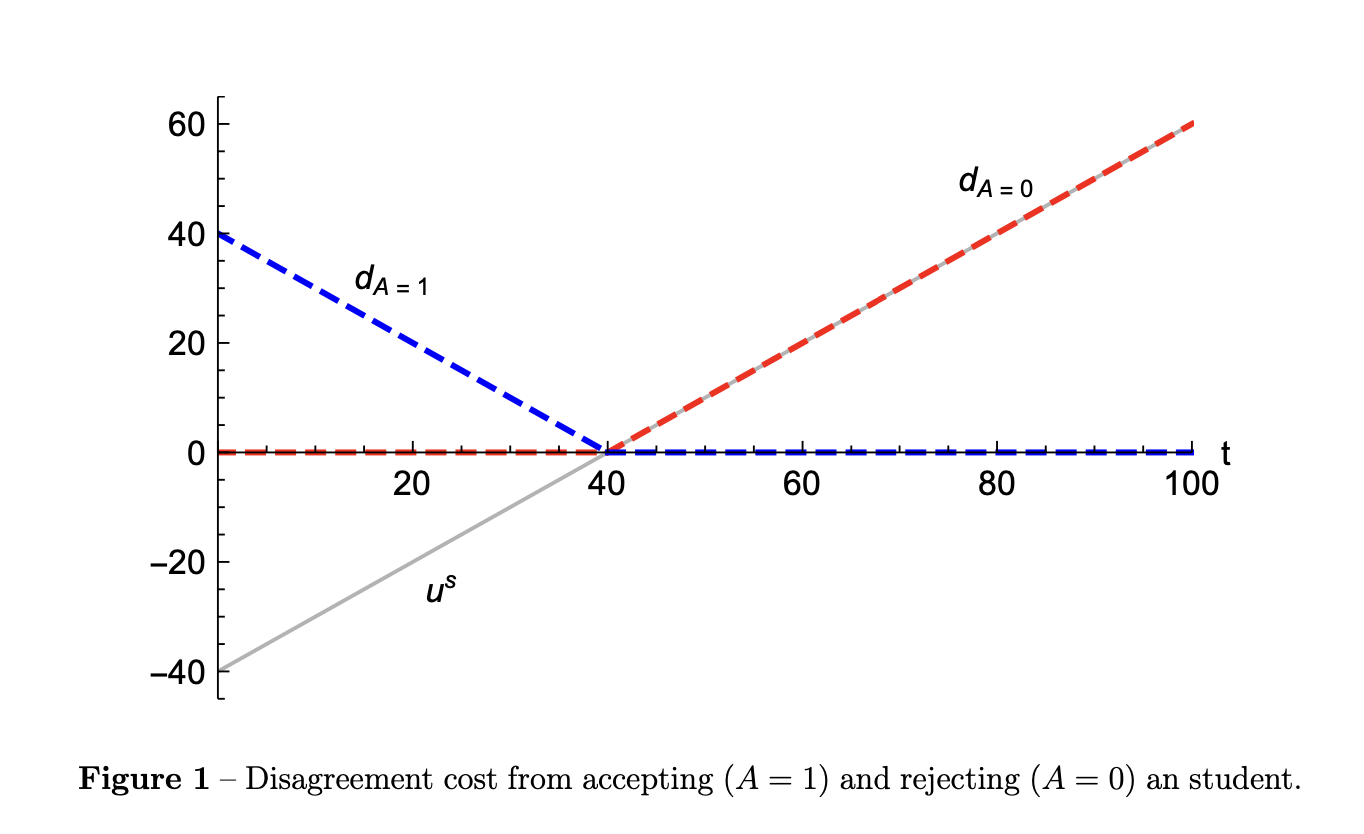
\includegraphics[width=0.65\textwidth]{testoptional-fig1.png} \end{center}
\end{frame}

% \begin{frame}
%     \centering
%     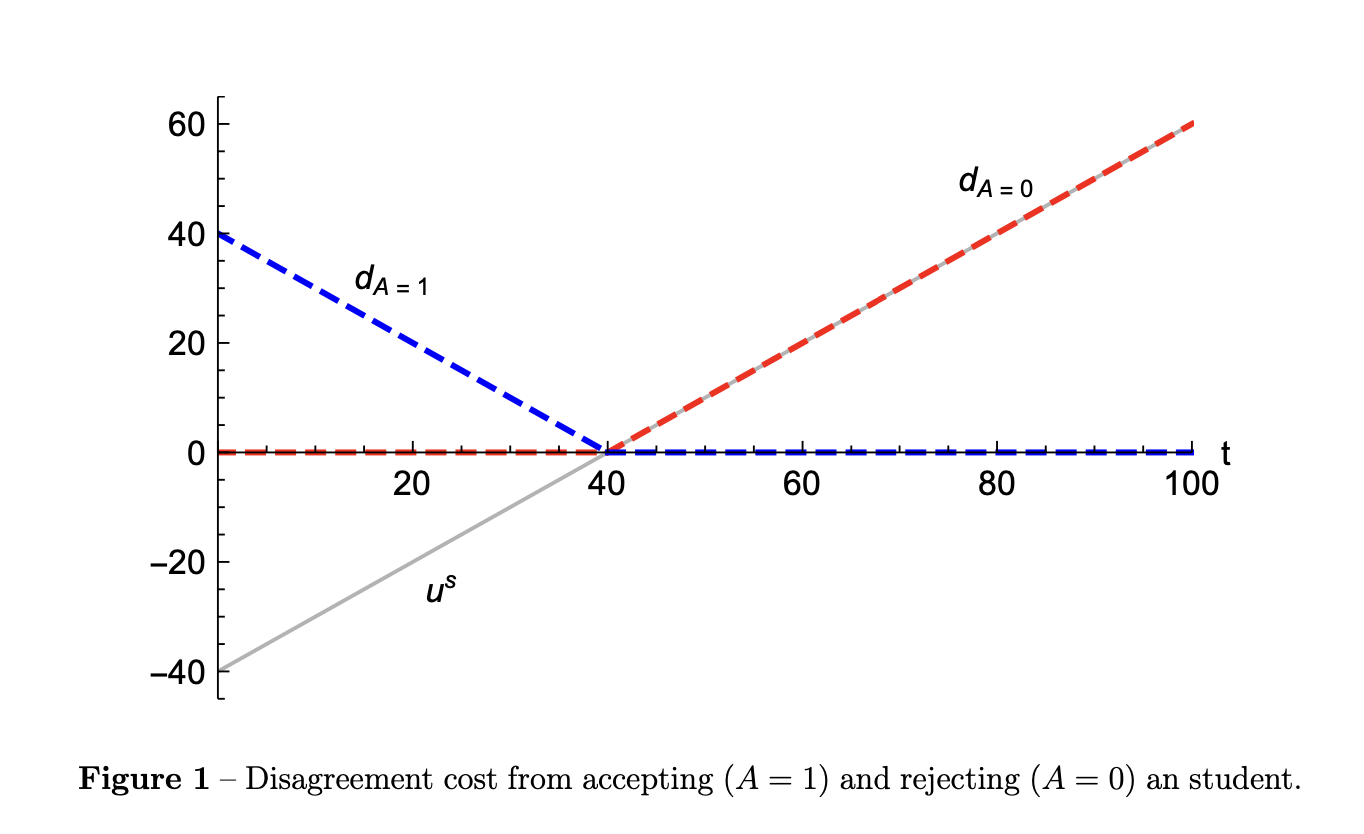
\includegraphics[width=\textwidth]{testoptional-fig1.png}
% \end{frame}

% \begin{frame}{Test-blind: motivated by inequality}\framesubtitle{Jensen's inequality}

% [draw picture here]

%  [specialize picture to case of college not caring about SAT scores]

%  [work example w/ picture, in which college cares zero about SAT scores]

%  [Rest of paper: this goes through when college cares!]
    
% \end{frame}

\begin{frame}{Where do disagreement costs come from?}
    \pause
    \begin{itemize}
        \item Two features of disagreement costs: \pause
        \begin{enumerate}
            \item zero if college, society agree on (binary) decision, otherwise $\propto$ |disagreement|. \pause
            \item Evaluated at expected value | available info. \pause
        \end{enumerate}
        \item $\implies$ Not simply college's preferences over entering class $\neq$ society's.  \pause
        \item ``social pressure'' term constant in region of agreement: \pause
        \item[] \ \ Stylized, but general shape may be very reasonable. \pause
        \begin{itemize}
            \item College gets little credit at margin for ``good'' decision; lots of blame for ``bad'' \pause
            \item $\implies$ Revealing ``extra'' info, beyond that needed for decision, runs risk of blame. \pause
            \item ``Ego utility'' (Koszegi 2006): to get a candidate not to learn own score, make payoff concave in E(score).  \pause
            %\item Reference dependence w/ normative reference could look like this.  \pause
            \item Journalism and litigation worse for colleges if there are obvious cases.
        \end{itemize}
    \end{itemize}
\end{frame}

\begin{frame}{How can colleges design society's information?}
    \begin{enumerate}
       \item Managing society's beliefs is easier if scores \emph{are not produced at all.} \pause
        \begin{itemize}
            \item should interpret college in this paper as coalition of all colleges (I think). \pause %one college closing its eyes is useless. 
            \item Aside: paper mentions 25 states (but not CA, NY) require SAT/ACT for high school graduation.  Couldn't society see these? \pause
            \item One exception (see end of this paper): SAT-blind may make some discriminination cases harder. \pause
        \end{itemize}

    \item Who controls the exam? \pause
        \begin{itemize}
            \item If run by a single elite college, why not make scores ``1'' or ``0''?  (Compare AP exams). \pause
            \item U.S. has competing private exams, unlike other countries w/ national college entrance exams.
        \end{itemize}
    \end{enumerate}
\end{frame}

\begin{frame}{Does competition among colleges matter?}
\begin{itemize}
    \item Empirical DiD lit is about individual small colleges dropping exams; this paper is about a monopolist. \pause
    \item Are SAT-optional decisions by colleges strategic complements? \pause
    \begin{itemize}
        \item If apps costly, not using SAT scores can induce more apps. \pause
        \item Value of taking SAT falls if fewer colleges use it. \pause
        \item If test-prep costly, then a college, $j$, going test-optional can reduce returns to effort for people who like $j$. \pause
    \end{itemize}
    \item Is world in 2023 very different from 2018? Maybe we want model with multiple eqba?
\end{itemize}
\end{frame}

\begin{frame}{Conclusions}
    \begin{itemize}
        \item This paper: colleges are designing the information that society uses to judge them, at some cost. \pause
        \begin{itemize}
            \item My view: worth pursuing this channel!
            \item Empirical lit: SAT-optional hasn't increased diversity or ability of entering class so far.
            \item This suggests that we should look for alternative explanations.  \pause
            \item Seems very plausible that colleges are trying to hide info used to make decisions. \pause
            \item This paper shows how to get this story to work in equilibrium. \pause 
            \item ``Disagreement costs'': RF for journalism, litigation, pressure from legislators, ...? \pause 
            \item Maybe we (empiricists) should think more about info design, e.g. how would we know if this is going on? \pause
        \end{itemize}
        \item A lot of interesting stories involve multiple firms:
        \begin{itemize}
            \item Many questions for next paper...
        \end{itemize}
        %oligopoly! many stories about why one college might adopt; are these decisions strategic complements? are there multiple eqba?
    \end{itemize}
\end{frame}

\end{document}


3.	Comments: "ways out of the puzzle"

	a. authors show some obvious ones don't work, e.g. model allows test prep effort; under complete lack of commitment, eqbm would probably unravel to full disclosure (but could imagine partial commitment, e.g. Texas Top Ten).

	b. If you ask colleges, they'll say it's to enlarge the applicant pool.  [quote from paper].
		*seemed to be first-order effect in TTT.
	    * of course, whether this "works" or not depends on good the college's non-exam info is, and what it does with it.
	    	[can flood app pool w/ bad applicants; hard to do initial screening; might be costly or lead to mismatches]
	    	[but if the college is very good at evaluating other parts of application, it might want to do this to get more draws.]
	    * why might dropping SAT enlarge the applicant pool?
			* Paper acknowleges: additional costs (e.g. sending exam; sitting for exam); non-eqbm behavior.
			* what about...

4. What about:
	A. oligopoly
	* two colleges, not 1.
	* applicants pick portfolios
	* [example w/ 2 colleges, one goes test-blind. w/ endog. effort, this might affect decisionmaking]
	(2 colleges: h ~ unif[0,1], t ~ F(e), c(e)=e ... )
	*  (for simplicity, can apply to at most 1).

	B. uncertainty about what the college wants:
		more likely to apply to colleges where you feel more wanted ("fit", admissions chance)
		if uncertainty about what Harvard wants, committing to "test optional" reveals it will want to accept some students w low scores ("whose strengths are not SAT scores")
		this can induce applications

5. Comments: 





N. Conclusion
  *something about theory/empirics